\documentclass[10pt,a4paper]{article}
\usepackage[a4paper,margin=1.3cm,top=1.0cm,bottom=1.1cm]{geometry}
\usepackage[T1]{fontenc}
\usepackage{mathpazo}
\usepackage[scaled=0.92]{helvet}
\usepackage{microtype}
\usepackage{booktabs,tabularx,array}
\usepackage{xcolor}
\usepackage{graphicx}
\usepackage{tikz}
\usetikzlibrary{positioning,arrows.meta,calc}
\usepackage{titlesec}
\usepackage{enumitem}
\usepackage[hidelinks]{hyperref}
\usepackage{caption}

\titleformat{\section}{\sffamily\bfseries\normalsize\color{teal!55!black}}{\thesection}{0.5em}{}
\titlespacing*{\section}{0pt}{5pt}{2pt}
\setlength{\parindent}{0pt}
\setlength{\parskip}{2pt}
\setlist{nosep,leftmargin=1.1em,topsep=1pt}
\captionsetup{font=footnotesize,labelfont=bf,skip=2pt}
\setlength{\textfloatsep}{6pt}
\setlength{\floatsep}{5pt}
\setlength{\intextsep}{5pt}
\setlength{\tabcolsep}{4pt}
\newcommand{\gr}[1]{\textcolor{black!55}{#1}}
\pagestyle{empty}

\begin{document}
\small

{\sffamily\bfseries\Large Lumbar spine L1--L5 segmentation from CT}\\[2pt]
{\footnotesize Take-home assignment report. Code, model weights and inference are in \texttt{lumbar/}; one command runs inference:
\texttt{./run\_inference.sh <input\_dir> <output\_dir>} (Python 3.10--3.12, CPU only, no GPU or Docker; tested on Windows~11, plain bash, about 20\,s per CT).}

\section{Overview}
We built one pipeline for lumbar CT (Fig.~\ref{fig:pipeline}). It standardises scans from two datasets, segments the vertebrae L1--L5 with a 3D network trained from scratch on TotalSegmentator, finds the centre of each vertebral body, and tests how well the model transfers to the VerSe dataset.
On typical cases the model is as accurate as the 2\,mm working resolution allows: the median Dice is 0.93 on TotalSegmentator and 0.92 on VerSe, against a limit of 0.94. The lower means come from a few scans where the vertebrae are found but misnamed.

\begin{figure}[h]
\centering
\resizebox{0.74\linewidth}{!}{% Pipeline overview for the short report: training (top row) and inference (bottom row)
% use the same "standardise" step, so the network sees the same kind of input in both.
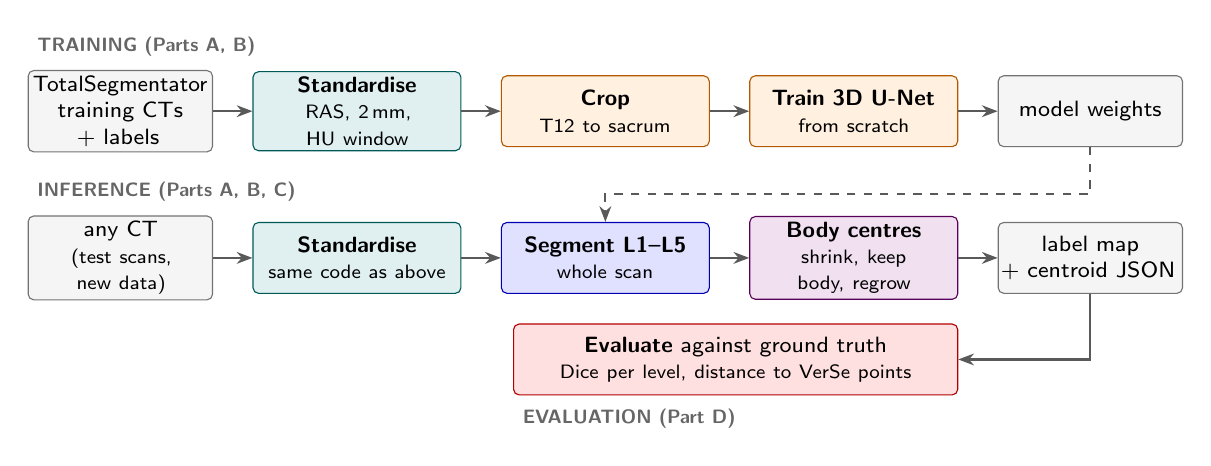
\begin{tikzpicture}[
    font=\sffamily\footnotesize,
    node distance=4mm and 5mm,
    step/.style={draw=#1!70!black, fill=#1!12, rounded corners=2pt, align=center,
                 minimum height=9mm, text width=25mm, inner sep=2pt},
    io/.style={draw=black!55, fill=black!4, rounded corners=2pt, align=center,
               minimum height=9mm, text width=22mm, inner sep=2pt},
    arr/.style={-{Stealth[length=2mm]}, thick, black!65},
    lane/.style={font=\sffamily\scriptsize\bfseries, text=black!60, anchor=south west},
  ]
  % training row
  \node[io] (tsin) {TotalSegmentator\\ training CTs + labels};
  \node[step=teal, right=of tsin] (std1) {\textbf{Standardise}\\ \scriptsize RAS, 2\,mm, HU window};
  \node[step=orange, right=of std1] (crop) {\textbf{Crop}\\ \scriptsize T12 to sacrum};
  \node[step=orange, right=of crop] (train) {\textbf{Train 3D U-Net}\\ \scriptsize from scratch};
  \node[io, right=of train] (weights) {model weights};

  % inference row
  \node[io, below=8mm of tsin] (ctin) {any CT\\ \scriptsize (test scans, new data)};
  \node[step=teal, right=of ctin] (std2) {\textbf{Standardise}\\ \scriptsize same code as above};
  \node[step=blue, right=of std2] (seg) {\textbf{Segment L1--L5}\\ \scriptsize whole scan};
  \node[step=violet, right=of seg] (body) {\textbf{Body centres}\\ \scriptsize shrink, keep body, regrow};
  \node[io, right=of body] (out) {label map\\ + centroid JSON};

  % evaluation
  \node[step=red, below=3mm of body, text width=55mm, xshift=-15mm] (eval)
       {\textbf{Evaluate} against ground truth\\ \scriptsize Dice per level, distance to VerSe points};

  \draw[arr] (tsin) -- (std1);
  \draw[arr] (std1) -- (crop);
  \draw[arr] (crop) -- (train);
  \draw[arr] (train) -- (weights);
  \draw[arr] (ctin) -- (std2);
  \draw[arr] (std2) -- (seg);
  \draw[arr] (seg) -- (body);
  \draw[arr] (body) -- (out);
  \draw[arr, dashed] (weights.south) |- ($(seg.north)+(0,3.5mm)$) -- (seg.north);
  \draw[arr] (out.south) |- (eval.east);

  \node[lane] at ($(tsin.north west)+(0,0.5mm)$) {TRAINING (Parts A, B)};
  \node[lane] at ($(ctin.north west)+(0,0.5mm)$) {INFERENCE (Parts A, B, C)};
  \node[lane, anchor=north west] at ($(eval.south west)+(0,-0.5mm)$) {EVALUATION (Part D)};
\end{tikzpicture}
}
\caption{Pipeline. Training and inference use the same standardisation code, so the network sees the same kind of input in both.}
\label{fig:pipeline}
\end{figure}

\section{Data and preprocessing (Part A)}
\textbf{Data.} TotalSegmentator v3 (1939 CTs) with its official split: 1830 training and 109 test scans. VerSe 2019 (validation and test sets, 80 CTs) is used only for testing, so it stays a truly unseen dataset. One loader reads both datasets.

\textbf{Three steps}, the same for both datasets and for training and inference.
(1)~\emph{Orientation}: image and labels are resampled onto a grid in RAS orientation using their affine matrix. This handles any axis order, flip or tilt at once.
(2)~\emph{Spacing}: 2\,mm in every direction. The CT is smoothed before it is downsampled; labels use nearest-neighbour interpolation.
(3)~\emph{Intensity}: Hounsfield units (HU) are clipped to a fixed window of $-1000$ to $1500$ and scaled to [0,\,1]. A fixed window, unlike per-scan normalisation, gives bone the same value in every scan, whatever the field of view.

\textbf{Anomalies.} An automatic check reads every header and label file and looks for 30 kinds of problems; Table~\ref{tab:anom} lists those that occurred. Checks of the output: structure centres move a median of 0.3\,mm, and side views of all scans show the correct orientation.

\begin{table}[h]
\centering\footnotesize
\caption{Anomalies found (number of scans; TS = TotalSegmentator, 1939; VS = VerSe19, 80). Checked but never found: conflicting qform/sform, tilted axes, zero voxel size, 4D images, NaN.}
\label{tab:anom}
\begin{tabularx}{\linewidth}{@{}l>{\raggedright\arraybackslash}X>{\raggedright\arraybackslash}Xrr@{}}
\toprule
Anomaly & How detected & How handled & TS & VS\\
\midrule
Image not stored axially (PIR, PSR, LAS) & orientation codes of the affine & resampled to RAS & 0 & 48\\
Thick slices (up to 3\,mm, 3$\times$ the in-plane size) & voxel sizes & smoothed before downsampling & 0 & 4\\
Only qform or only sform set & header codes & use the one that is set & 1939 & 80\\
CT stored as float, HU not whole numbers & data type and values & accepted (resampled by provider) & 0 & 77\\
Label and CT affines differ by $\le$\,0.001\,mm & affine difference & treated as the same grid & 228 & 36\\
Label mask stored as float & data type & rounded to whole numbers & 0 & 1\\
\midrule
Two masks claim the same voxel (mostly S1 and L5) & overlap of the masks & the lumbar level wins & 817 & 0\\
Padding below $-2000$\,HU outside the scan circle & share of such voxels & set to air by the HU window & 104 & 0\\
Metal near the spine & $>$\,0.5\,ml above 3000\,HU & clipped at 1500\,HU, flagged & 124 & 4\\
Vertebra cut off by the scan edge & mask touches the border & kept; Dice also reported without them & 431 & 8\\
No lumbar vertebra in the scan & label content & excluded from training & 720 & 13\\
Sixth lumbar vertebra (L6) & VerSe label 25 & own class, never merged into L5 & 0 & 3\\
\bottomrule
\end{tabularx}
\end{table}

\section{Model and training (Part B)}
\textbf{Network.} We use the residual-encoder U-Net (``ResEnc M'', 102\,M parameters) from Isensee et al., \emph{nnU-Net Revisited} (MICCAI 2024), trained from scratch. In their benchmark, where all models were trained from scratch with the same budget, this CNN beat Transformer- and Mamba-based networks. We use only the network, not the full nnU-Net framework: the framework would replace our own preprocessing, and its default mirroring along every axis would swap L1 and L5.

\textbf{Training data.} The network predicts L1--L5 plus T12 and the sacrum; the two extra classes are fixed landmarks that help it count the levels. Training uses crops from T12 to the sacrum with a 3\,cm margin. Crops without a lumbar level, or with only a tiny piece of one ($<$\,2\,ml), were removed. This leaves 902 training and 100 validation scans; the official test split is never used. Patches of 96$\times$96$\times$160 voxels (19$\times$19$\times$32\,cm) contain T12 to the sacrum, so the network sees the whole lumbar spine at once.

\textbf{Training setup.} Loss: cross-entropy plus Dice. Optimiser: the nnU-Net defaults without change (SGD, learning rate 0.01 with polynomial decay), so nothing was tuned by hand. No data augmentation: flips would swap levels or mirror the anatomy, and about 900 scans are enough for a short run. Training ran for 11\,000 steps (batch size 8, mixed precision) in 2.6\,h on one RTX~3090. We kept the checkpoint with the best validation Dice (0.90, at step 8000). At inference the network runs over the whole scan in overlapping windows. For each level only the largest connected piece is kept, and the result is mapped back to the original CT grid.

\section{Vertebral body centroid (Part C)}
\textbf{Method.} The vertebral body is the only part of a vertebra that is thicker than about 12\,mm; the pedicles, laminae and processes are thinner. We therefore
(1)~shrink the vertebra mask by 6\,mm, which removes all thin parts,
(2)~keep the largest remaining piece that is not behind the centre of the vertebra,
(3)~grow it back by 6\,mm, but only inside the original mask, and
(4)~take its centre of mass in world coordinates (RAS, mm) (Fig.~\ref{fig:body}).
It uses only the shape of the bone, not a fixed cutting plane, so it works for any patient position and vertebra size. If nothing survives step~1 (small pieces cut off by the scan edge), the whole-vertebra centre is used (32 of 642 vertebrae).

\textbf{Validation.} VerSe provides one annotated point per vertebra. These points lie a median of 11.7\,mm in front of the centre of the whole vertebra, so they mark the centre of the \emph{body} and can serve as a reference. On the VerSe ground-truth masks, our body centre lies a median of \textbf{0.9\,mm} from the annotated point (90th percentile 3.9\,mm), compared with 12.5\,mm for the centre of the whole vertebra. On the predicted masks the distance is 1.0\,mm (90th percentile 7.5\,mm). The rule ``not behind the centre'' was added after inspecting VerSe outliers; no other setting was adjusted on VerSe.

\begin{figure}[h]
\centering
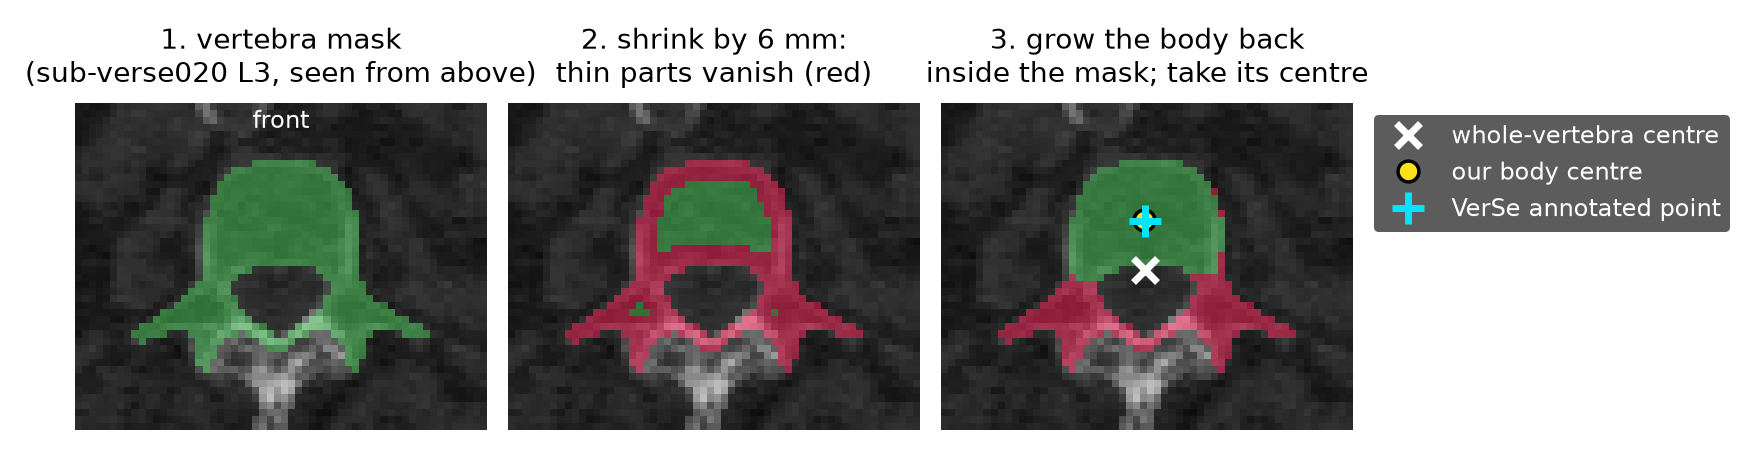
\includegraphics[width=0.52\linewidth]{figures/body_centre_steps.png}
\caption{Finding the body centre on one slice (green: kept, red: removed). Our body centre lies on the VerSe point; the whole-vertebra centre lies behind the body.}
\label{fig:body}
\end{figure}

\section{Cross-dataset evaluation (Part D)}
\textbf{Label mapping.} TotalSegmentator \texttt{vertebrae\_L1}--\texttt{L5} and VerSe labels 20--24 both become L1--L5. Transitional vertebrae (VerSe 25 = L6, 28 = T13) keep their own classes, so they are never counted as L5, T12 or background.
\textbf{Scoring.} Dice is computed on the original CT grid, only for levels that exist in the ground truth (tiny label pieces $<$\,2\,ml are excluded). Levels predicted where the ground truth has none are counted separately as false positives. These rules were fixed before seeing the results.

\begin{table}[h]
\centering\footnotesize
\caption{Dice per vertebra, mean / median; $n$ = scored vertebrae. \emph{Limit}: ground truth resampled to 2\,mm and back; no 2\,mm model can do better.}
\label{tab:dice}
\begin{tabular}{@{}lccccccc@{}}
\toprule
Test set & L1 & L2 & L3 & L4 & L5 & All & $n$\\
\midrule
TotalSegmentator test (in-domain, 78 scans) & .86 / .93 & .88 / .93 & .89 / .93 & .90 / .93 & .88 / .92 & \textbf{.88 / .93} & 328\\
VerSe19 (out-of-domain, 67 scans) & .85 / .92 & .85 / .92 & .86 / .92 & .86 / .92 & .84 / .91 & \textbf{.85 / .92} & 305\\
\gr{Limit (both test sets)} & \gr{.94} & \gr{.94} & \gr{.94} & \gr{.94} & \gr{.94} & \gr{.94} & \\
\bottomrule
\end{tabular}
\end{table}

\textbf{Why the results differ.} The medians are almost the same (0.93 and 0.92) and close to the limit of 0.94, so a typical vertebra is segmented equally well on both datasets. The means are lower because a few scans fail completely, and these failures are naming errors, not boundary errors (Fig.~\ref{fig:fail}):
\begin{itemize}
\item \emph{Wrong level count.} In 5 scans (1 TotalSegmentator, 4 VerSe), renaming all predicted levels by one raises the Dice by more than 0.1, for example from 0.00 to 0.67 in a scan with metal implants. Causes: metal, fractured vertebrae, and short scans without the sacrum or ribs as landmarks.
\item \emph{Cut-off vertebrae} are harder to segment and name; without them the TotalSegmentator mean rises from 0.88 to 0.91.
\item \emph{Domain shift.} VerSe has other scanners, thicker slices, more fractures and more metal. This barely changes typical cases but makes naming errors more frequent.
\end{itemize}

\textbf{Odd findings.}
\begin{itemize}
\item \emph{VerSe does not label vertebrae cut off by the scan edge; TotalSegmentator does.} On VerSe the model predicts 12 vertebra-sized levels missing from the ground truth; 8 touch the scan edge, and those inspected are real vertebrae. This is a labelling difference, not a model error.
\item \emph{False labels in scans without a lumbar spine.} All 27 such TotalSegmentator test scans receive small lumbar predictions (median 0.8\,ml). The model was trained on lumbar crops only and never saw a chest or a head.
\item \emph{Patients with L6} (3 VerSe scans) are handled correctly (Dice 0.87--0.94 per level): the model counts from the top, as VerSe does, and leaves L6 unlabelled.
\end{itemize}

\begin{figure}[h]
\centering
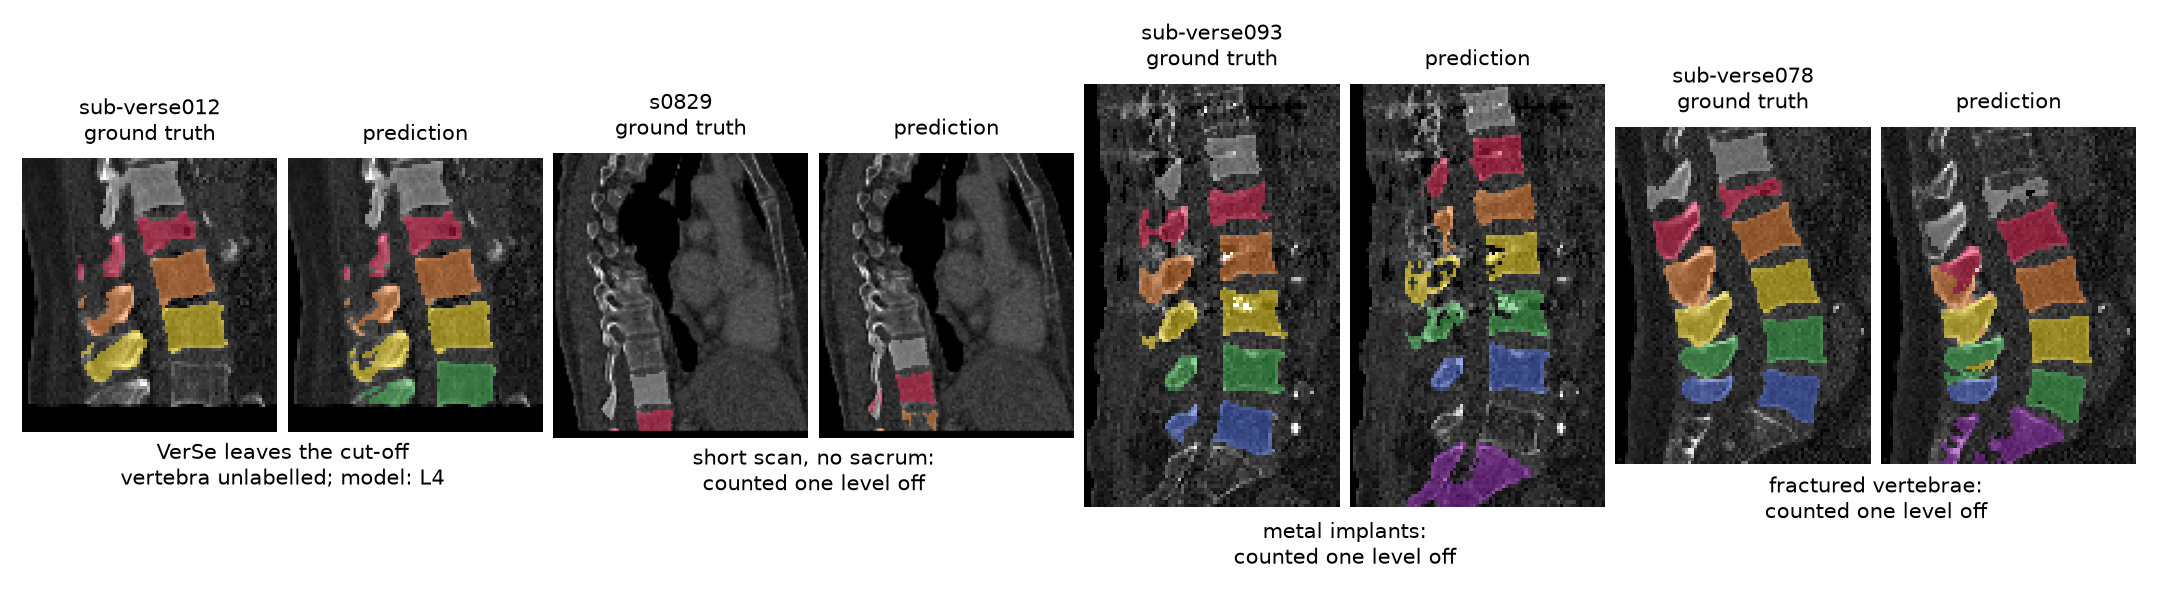
\includegraphics[width=0.85\linewidth]{figures/failure_cases_side_views.png}
\caption{Typical failures, side view (head up, front to the right): ground truth next to prediction. L1 red, L2 orange, L3 yellow, L4 green, L5 blue, T12 grey, sacrum purple.}
\label{fig:fail}
\end{figure}

\section{Next steps, and what we would not do}
\textbf{With more resources we would:}
(1)~check the level names with a simple rule (order the vertebrae from head to feet, with T12 and the sacrum as anchors) to fix the off-by-one errors;
(2)~add some patches from whole scans to training, or a ``lumbar spine present?'' check, to remove the false labels in non-lumbar scans;
(3)~score VerSe only on complete vertebrae, so both datasets follow the same labelling rule;
(4)~use cross-validation and confidence intervals, because 67--78 test scans is a small sample.

\textbf{We would deliberately not:}
train or tune on VerSe, because it would then no longer test transfer to an unseen dataset;
use a larger model to raise the Dice, because the medians are already near the 2\,mm limit and the remaining errors are naming and labelling differences;
train a network for the vertebral body, because no body labels exist and the shape rule is already within 1\,mm of the expert points.

\end{document}
